%\documentclass{scrartcl}
\documentclass{standalone}
\usepackage{tikz,ifthen}

%
% Customize colors
%
\definecolor{chapter-color}{cmyk}{1, 0.50, 0, 0.25}
\definecolor{link-color}{cmyk}{1, 0.50, 0, 0.25}
\definecolor{cite-color}{cmyk}{0, 0.7, 0.9, 0.2}
\definecolor{codegreen}{rgb}{0,0.6,0}
\definecolor{codegray}{rgb}{0.5,0.5,0.5}
\definecolor{codepurple}{rgb}{0.58,0,0.82}
\definecolor{backcolour}{rgb}{0.95,0.95,0.92}
\definecolor{codebgcolor}{RGB}{129, 139, 152}
\definecolor{codehighlightcolor}{RGB}{255, 230, 153}
%\definecolor{codegreen}{RGB}{0, 153, 0}
%\definecolor{codegray}{RGB}{127, 127, 127}
\definecolor{codeblue}{RGB}{102, 214, 237}
\definecolor{codekeyword}{RGB}{249, 36, 114}
\definecolor{codecomment}{RGB}{127, 127, 127}
\definecolor{backcolor}{RGB}{242, 242, 235}
\definecolor{linkcolor}{RGB}{102, 0, 0}
\definecolor{corange}{RGB}{255, 70, 0}
\definecolor{cyellow}{RGB}{209, 153, 0}
\definecolor{cblue}{RGB}{64, 128, 255}
\definecolor{cbrown}{RGB}{153, 102, 51}
\definecolor{cpink}{RGB}{255, 0, 255}
\definecolor{cred}{RGB}{255, 64, 0}
\definecolor{cgreen}{RGB}{0, 191, 0}
\definecolor{clightblue}{RGB}{191, 217, 255}
\definecolor{cturquois}{RGB}{0, 255, 255}
\definecolor{cpurple}{RGB}{128, 0, 255}
\definecolor{clightgreen}{RGB}{175, 255, 175}
\definecolor{clightgray}{RGB}{211, 211, 211}
\definecolor{clightpink}{RGB}{255, 175, 255}
\definecolor{cdarkblue}{RGB}{0, 0, 255}
\definecolor{cdarkred}{RGB}{255, 0, 0}
\definecolor{cdarkgreen}{RGB}{0, 255, 0}
\definecolor{cgray}{RGB}{153, 153, 153}

\definecolor{myblue}{RGB}{55, 126, 184}
\definecolor{myorange}{RGB}{255, 127, 0}
\definecolor{myred}{RGB}{228, 26, 28}
\definecolor{mypurple}{RGB}{152, 78, 163}
\definecolor{mygreen}{RGB}{77, 175, 74}
\definecolor{myyellow}{RGB}{255, 255, 51}
\definecolor{mybrown}{RGB}{166, 86, 40}
\definecolor{mypink}{RGB}{166, 86, 40}
\definecolor{mygray}{RGB}{153, 153, 153}


\tikzset{contr/.style={
    fill=cred!30!white,
    minimum height=20pt,
    minimum width=70pt,
    anchor=west}
}

\tikzset{solve/.style={
    fill=cblue!30!white,
    minimum height=20pt,
    minimum width=120pt,
    anchor=west}
}

\tikzset{plain/.style={
    fill=white,
    minimum height=20pt,
    minimum width=40pt,
    anchor=west}
}


\begin{document}
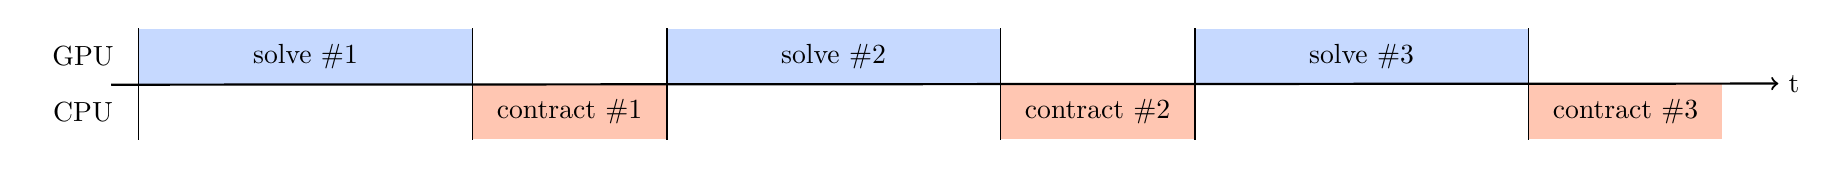
\begin{tikzpicture}

\node[plain] (gpu) at (0pt, 20pt) {GPU};
\node[plain] (cpu) at (0pt, 0pt)  {CPU};

\node[solve] (solve1) at (gpu.east) {solve \#1};
\node[contr] (contr1) at ([yshift=-20pt] solve1.east) {contract \#1};

\node[solve] (solve2) at ([yshift=+20pt] contr1.east) {solve \#2};
\node[contr] (contr2) at ([yshift=-20pt] solve2.east) {contract \#2};

\node[solve] (solve3) at ([yshift=+20pt] contr2.east) {solve \#3};
\node[contr] (contr3) at ([yshift=-20pt] solve3.east) {contract \#3};

\draw[thick,->] ([xshift=-10pt] solve1.south west) -- ([xshift=20pt] contr3.north east) node[right]{t};

\draw[thin,-] (solve1.north west) -- ([yshift=-20pt] solve1.south west);
\draw[thin,-] (solve1.north east) -- ([yshift=-20pt] solve1.south east);
\draw[thin,-] (solve2.north west) -- ([yshift=-20pt] solve2.south west);
\draw[thin,-] (solve2.north east) -- ([yshift=-20pt] solve2.south east);
\draw[thin,-] (solve3.north west) -- ([yshift=-20pt] solve3.south west);
\draw[thin,-] (solve3.north east) -- ([yshift=-20pt] solve3.south east);

\end{tikzpicture}
\end{document}
